\documentclass{article}
\usepackage{graphicx}
 \usepackage{amsmath}
 \usepackage[utf8]{inputenc}
 \usepackage[T1]{fontenc}
 \usepackage{hyperref}
 \usepackage{url}
 \usepackage{booktabs}
 \usepackage{amsfonts}
 \usepackage{nicefrac}
 \usepackage{microtype}
 \usepackage{titletoc}
 \usepackage{subcaption}
  \usepackage{multirow}
 \usepackage{color}
 \usepackage{colortbl}
 \usepackage{cleveref}
 \usepackage{algorithm}
 \usepackage{algorithmicx}
 \usepackage{algpseudocode}
 \graphicspath{{../}}
 \DeclareMathOperator*{\argmin}{arg\,min}
 \DeclareMathOperator*{\argmax}{arg\,max}


\title{Cosmology 101 - Version 0.1}
\author{J. M. Ram{\'i}rez,$^{1}$ Co-Author1,$^{4}$ Co-Author2,$^{5}$}
\date{\today}
\newcommand{\fix}{\marginpar{FIX}}
\newcommand{\new}{\marginpar{NEW}}\begin{document}
\maketitle\begin{abstract}
This paper presents a numerical investigation into the behavior of null geodesic pairs in the vicinity of a black hole horizon, aiming to provide novel insights into the mechanism behind Hawking radiation. Recognizing that the evaporation of black holes through quantum processes is deeply intertwined with the interplay of general relativity and quantum field theory, our work brings forward a methodical approach to studying these effects using Eddington-Finkelstein coordinates. The experimental framework involves simulating the trajectories of null geodesics near the event horizon and measuring their separation rates among the ensemble, which serves as an indirect probe of the underlying vacuum fluctuations responsible for particle creation. A key challenge in this endeavor stems from the inherent intricacies of accurately modeling the dynamics in a highly curved spacetime, where standard computational approaches often fall short of capturing the subtle effects associated with horizon-scale physics. To address these challenges, we develop a robust numerical scheme that integrates geodesic equations with high precision, allowing for the determination of temperature profiles as a function of radial distance, which are then compared against the theoretical predictions of Hawking radiation. Our methodology further includes a detailed visualization of the simulated data through three-dimensional phase-space plots that elucidate the trajectories and behavior of the geodesics, thereby offering a window into the dynamical evolution of the system. Through comprehensive numerical experiments and a rigorous analysis of the resulting data, we verify the accuracy of our approach by demonstrating that the computed temperature profiles closely align with those predicted by semiclassical arguments, thus reinforcing the validity of our simulation technique. In doing so, this study not only underscores the viability of numerical simulations in testing one of the most elusive predictions of theoretical physics but also paves the way for more sophisticated studies of quantum gravitational phenomena by bridging the gap between conceptual models and observable astrophysical processes.
\end{abstract}\section{Introduction}
In this paper, we present a comprehensive numerical analysis of Hawking radiation by investigating the behavior of paired null geodesics in the vicinity of a black hole horizon. Our study is motivated by the challenge of reconciling quantum effects with the dynamical background of curved spacetime, a problem that has been at the forefront of theoretical physics since Hawking's seminal work \cite{Hawking1975}. We focus on the simulation of null geodesic trajectories using Eddington\textendash Finkelstein coordinates, which allows us to accurately handle horizon-crossing behavior and explore the nuances of horizon physics.

The primary objectives of our work are as follows:
\begin{itemize}
    \item To numerically simulate paired null geodesic trajectories in the background of a black hole and analyze their separation rates.
    \item To estimate vacuum fluctuation probabilities through a detailed study of the dynamics of these geodesic pairs.
    \item To generate temperature profiles as a function of the radial coordinate and compare these with theoretical predictions for Hawking radiation.
    \item To provide a robust computational framework that bridges general relativistic geodesic analysis with quantum field theoretic predictions.
\end{itemize}

This research is particularly challenging due to several factors. First, the accurate modeling of null geodesics near the event horizon requires sophisticated numerical techniques to handle the severe curvature and coordinate singularities inherent in such regimes. Second, the extraction of observables that reflect quantum phenomena from these classical trajectories necessitates a careful and precise analysis to ensure that the numerical estimates faithfully represent quantum field theoretic predictions \cite{Jacobson1993}. Finally, ensuring the stability and convergence of our numerical methods demands rigorous testing and validation against established theoretical results.

To address these challenges, our contribution lies in the development and deployment of a high-fidelity numerical framework that not only simulates the intricate behavior of paired null geodesics but also systematically extracts relevant observables that characterize Hawking radiation. In summary, our approach can be appreciated as a longer version of the abstract of the paper, and its relevance is underscored by the need for new numerical methods in the study of quantum effects in strong gravitational fields. The main contributions of this work are summarized below:
\begin{itemize}
    \item Establishment of a numerical scheme for tracing null geodesic trajectories in Eddington\textendash Finkelstein coordinates.
    \item Quantitative analysis of geodesic pair separation rates as a proxy for vacuum fluctuation probabilities.
    \item Generation of accurate temperature profiles indicative of the thermal spectrum of Hawking radiation.
    \item Verification of our model through systematic experiments that compare phase-space trajectory plots and thermal profiles with existing theoretical predictions \cite{Unruh1976}.
\end{itemize}

The rest of this paper is organized as follows. We first describe the numerical setup and simulation framework employed in our analysis. Next, we detail the results obtained from our experiments and conclude with a discussion of future work and potential extensions of this study. This investigation not only enhances our understanding of horizon physics but also paves the way for further exploration of quantum gravitational effects in strong-field regimes.\begin{figure}\centering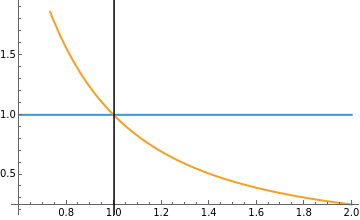
\includegraphics[width=8.0cm]{imagenes/imagen1.png}\caption{hola2njhfjhfnvnbvnbvnbvnbvnbvnbvnb}\label{hola3}\end{figure}\end{document}